\section{Properties of the Communities Core}

Next, we present a series of analyses about the scientific communities core. First, we analyze the network properties of scientific communities evolution in Section~\ref{sub:time}.
Then, Section~\ref{sub:vs} contrasts the properties of the communities core over time against the properies of the remaining communities authors. Then, in
Section~\ref{sub:avg_core} we compute the average core score of a community to investigate variations properties of the members of the core of each community. Finally,
Section~\ref{sub:corr} correlates these variations with the network properties of the communities. 


\subsection{Communities Evolution}
\label{sub:time}

As an attempt to understand the main structural properties of the scientific communities, next we examine the evolution of the structure of their networks on the light of complex
network analysis. To do so, we calculated various network metrics for each of the scientific communities. We present four popular metrics here: assortativity, average clustering
coefficient, average path length, and the size of the largest connected component.  Figure~\ref{fig:metrics_accumulated_1_in_1} shows how each of these four metrics vary over time
for a set of six scientific communities selected among those that spam over the longest period in our dataset.  Our analysis are performed under two perspectives. The first
consists on analyzing the network evolution year by year of accumulating nodes and edges to a single final snapshot of the graph. This perspective allow us to observe the final
network structure of a community as a function of time. The second perspective consists of analyzing snapshots constructed based on nodes and edges created on an predefined time
window (three years, as discussed in Section~\ref{sub:thresholds}). This analysis allow us to investigate network variations with potential to impact the final network structure.
Our analysis results are similar for the other communities, but we omit
them due to lack of space.

We can note from Figure~\ref{fig:metrics} that the largest connected component tend to largely increase as a function of time. This suggests that at early
stages, scientific communities are formed by several small and segregated research groups. With time, some reserachers (e.g., students) leave an institute and begin collaborations
with other research groups. Additionally, as the community evolves, heads of  research groups tend to colabrate with other peers of the same community. Thus, with time, authors
from different groups tend to collaborate and increase the size of the largest connected component. As a consequence, the average shortest path, computed only on the largest
connected component, tends to increase, becoming stable around typical small-world values (i.e., from 4 to 10 hops)~\cite{mislove-2007-socialnetworks,fourdegrees_facebook}.  We can
also note that the average clustering coefficient tends to values between 0.1 and 0.2, thus suggesting that the coauthors of an author have 10\% to 20\% of chance to be connected
among themselves. These values tend to slightly diminishe over time, as small components tend to connect to form larger components reducing the average clustering coefficient
value.  When it comes to assortativity, we see that this measure tends to 0, but it is still positive. This means that there is a slight tendency in these communities of nodes to
connect with others with similar degree.  A positive value for assortativity is a typical characteristic of sociological networks~\cite{Newman2003}.

In general, we can note that scientific communities have similar evolving characteristics and these properties are dynamic as they change over time.  More important, our
observations suggest that a small set of authors are responsible for the social clue that create the paths among smaller and more connected research groups. Next, we seek to
further investigate this group of authors. To that end, in the next section we propose an approach to identify the authors' core of scientific communities.



\begin{figure}[!htb]
  \begin{center}
  \subfigure[Final Assortativity]{%
    \label{fig:assortativity_1_in_1}
    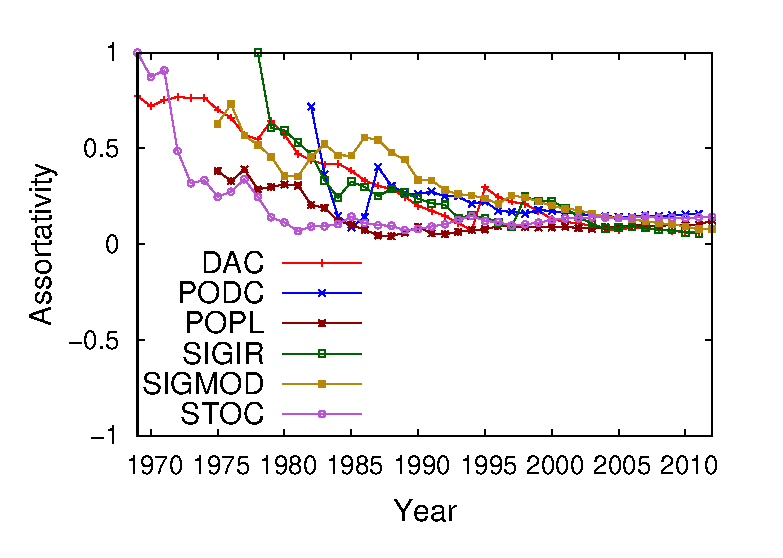
\includegraphics[scale=.33]{graficos/sigs_metricas_acumuladas_1_em_1_ano/assortatividade_grupo_temporal_web.eps}
  }%
  \subfigure[Assortativity per Window]{%
    \label{fig:assortativity_slide_window}
    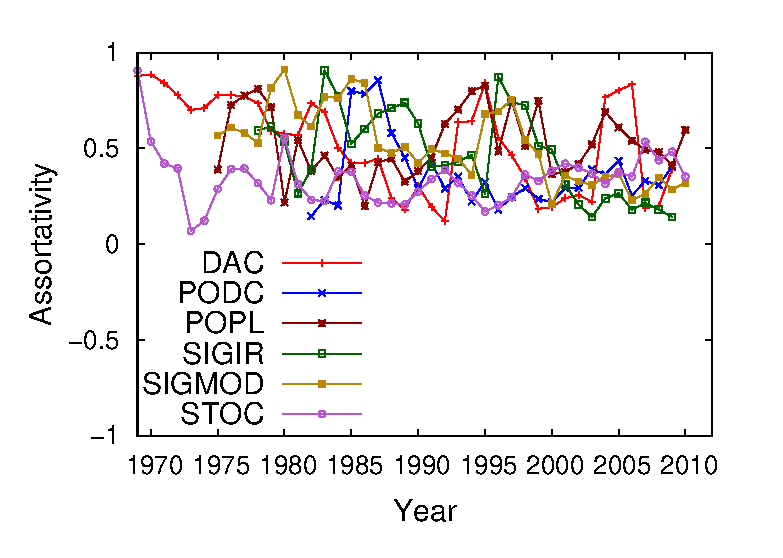
\includegraphics[scale=.33]{graficos/core_over_time/metricas_tradicionais/assortatividade_slide_window_grupo_temporal_web.eps}
  }%
  \\
  \subfigure[Final average shortest path]{%
    \label{fig:average_shortest_path_1_in_1}
    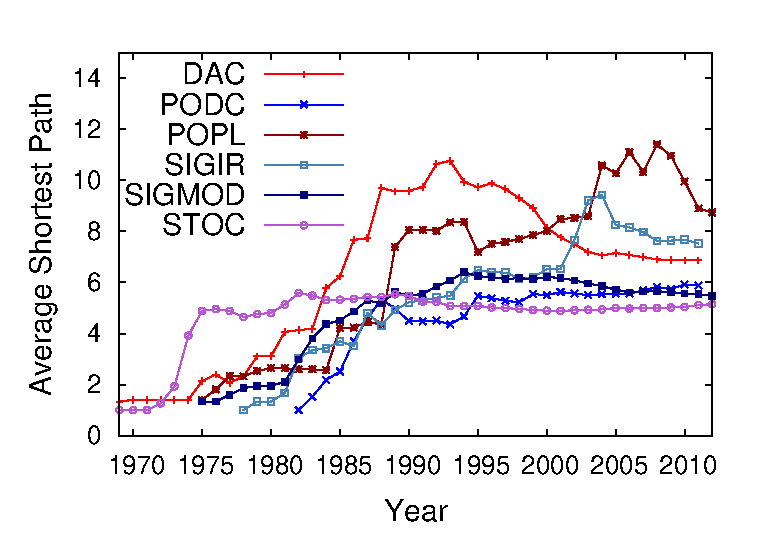
\includegraphics[scale=.33]{graficos/sigs_metricas_acumuladas_1_em_1_ano/caminho_minimo_medio_grupo_temporal_web.eps}
  }%
  \subfigure[Avg. shortest path per window]{%
    \label{fig:average_shortest_path_slide_window}
    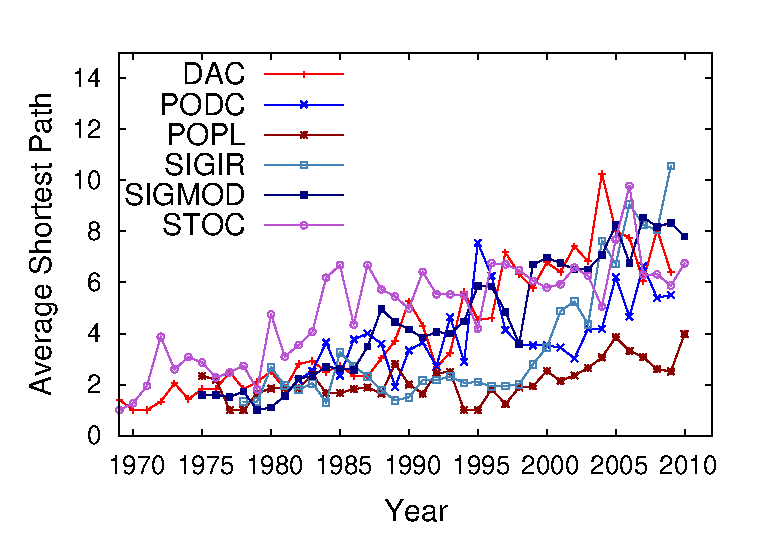
\includegraphics[scale=.33]{graficos/core_over_time/metricas_tradicionais/caminho_minimo_medio_slide_window_grupo_temporal_web.eps}
  }%
  \\
  \subfigure[Final clustering coefficient]{%
    \label{fig:clustering_coefficient_1_in_1}
    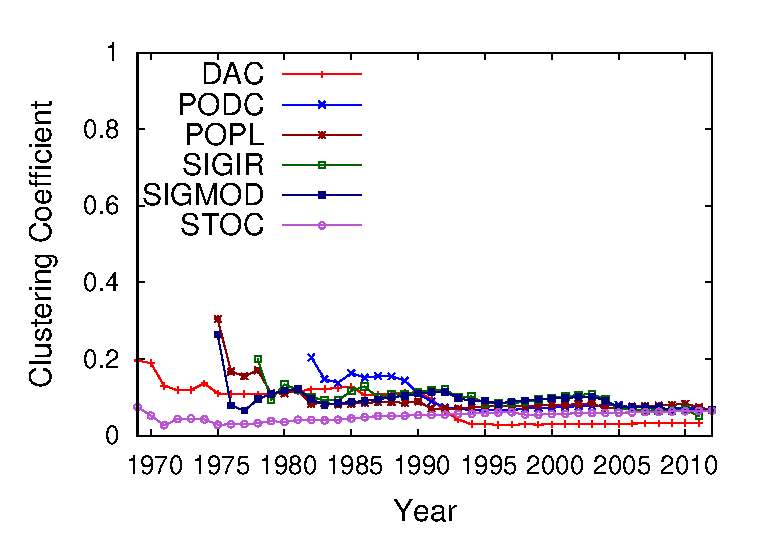
\includegraphics[scale=.33]{graficos/sigs_metricas_acumuladas_1_em_1_ano/coeficiente_agrupamento_grupo_temporal_web.eps}
  }%
  \subfigure[Clustering coefficient per window]{%
    \label{fig:clustering_coefficient_slide_window}
    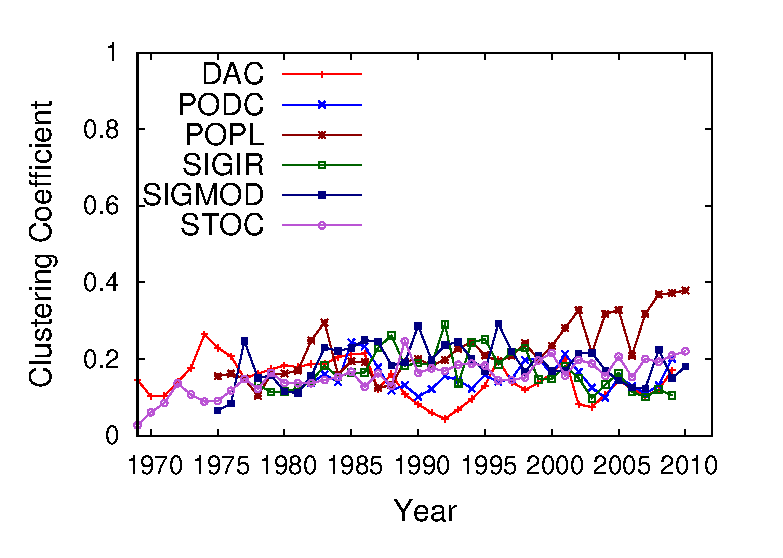
\includegraphics[scale=.33]{graficos/core_over_time/metricas_tradicionais/coeficiente_agrupamento_slide_window_grupo_temporal_web.eps}
  }%
  \\
  \subfigure[Final largest connected component]{%
    \label{fig:largest_connected_component_1_in_1}
    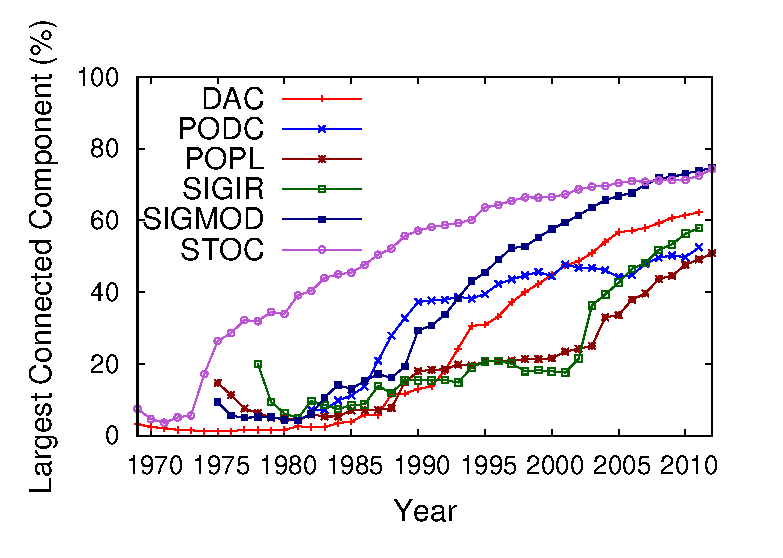
\includegraphics[scale=.33]{graficos/sigs_metricas_acumuladas_1_em_1_ano/porcentagem_maior_componente_grupo_temporal_web.eps}
  }%
  \subfigure[Largest connected component per window]{%
    \label{fig:largest_connected_component_slide_window}
    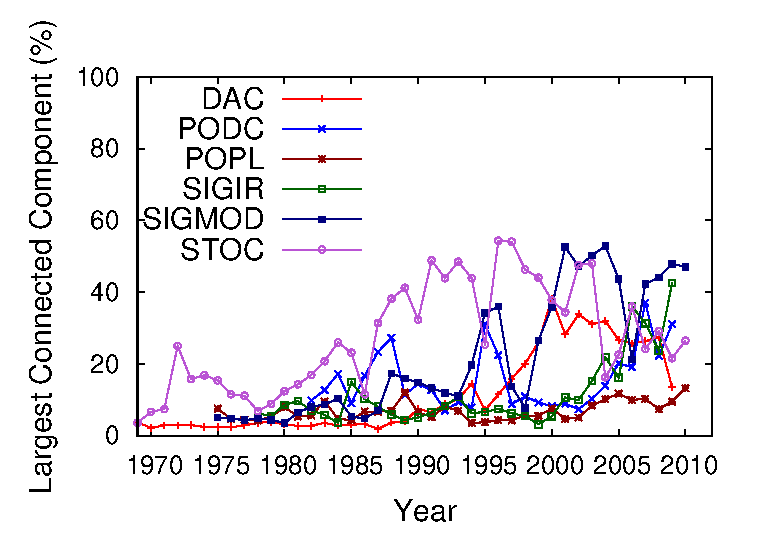
\includegraphics[scale=.33]{graficos/core_over_time/metricas_tradicionais/porcentagem_maior_componente_slide_window_grupo_temporal_web.eps}
  }%
  \\
  \subfigure[Final average degree]{%
    \label{fig:average_degree_1_in_1}
    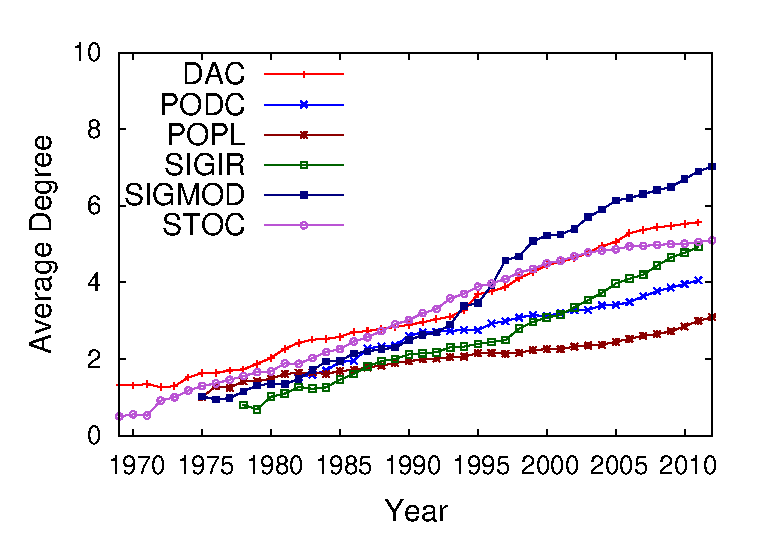
\includegraphics[scale=.33]{graficos/sigs_metricas_acumuladas_1_em_1_ano/grau_medio_nodos_grupo_temporal_web.eps}
  }%
  \subfigure[Avg. degree per window]{%
    \label{fig:average_degree_slide_window}
    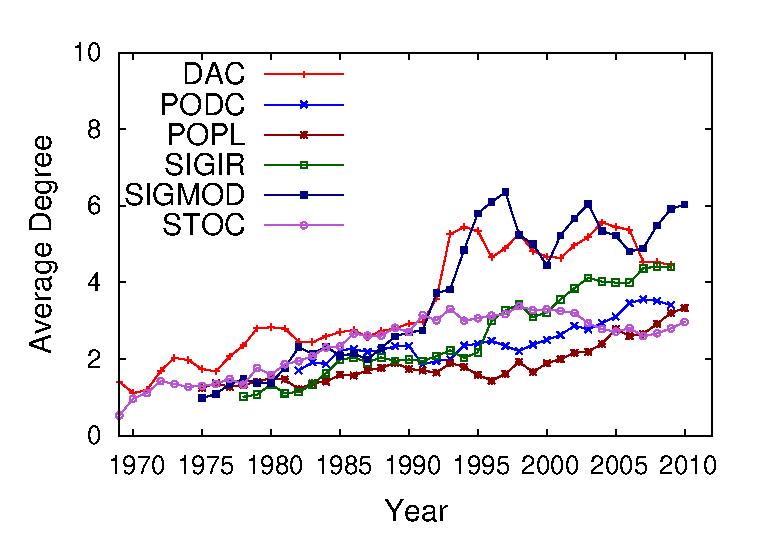
\includegraphics[scale=.33]{graficos/core_over_time/metricas_tradicionais/grau_medio_nodos_slide_window_grupo_temporal_web.eps}
  }%
  \end{center}
  \caption{Network evolution metrics for scientific communities}
  \label{fig:metrics}
\end{figure}

All in all, we can note that scientific communities have similar evolving characteristics and these properties are dynamic as they change over time.  More important, our
observations suggest that a small set authors are responsible for the social clue that create the paths among smaller and more connected research groups. Next, we seek to further
investigate this group of authors. To that end, in the next section we propose an approach to identify the author's core of scientific communities.

\if 0
Thus as the communities, the core community also evolves over the years. The Figure \ref{fig:metrics_accumulated_1_in_1}
showns how the communities evolves over the time considering data accumulated. Here, we show a different way to see the evolution,
the Figure \ref{fig:metrics_slide_window} showns the evolution of the communities over the year over the years using temporal slide 
window. It is possible to clearly see some differences, as the assortativity in Figure \ref{fig:assortativity_1_in_1}
and Figure \ref{fig:assortativity_slide_window} which in the first one, it start at 1 in many cases and stabilizes at 0 
nowadays, however, the slide windows show a large variation over the time, this may indicate, peharps, that the community come by
more variation than expected. This vision is so important to understand the core community, how we are explaing.\\
\fi 

\subsection{Core vs. Other Members}
\label{sub:vs}

So, to what extend the properties of the core community differ from the rest of the community?  Next, we compute node network properties for members and non-members of the core
community. We consider the time window analysis to understand the variations that these two classes might have in the global measure.
Figure~\ref{fig:metrics_comparing_core_community} shows the average degree and the average clustering coefficient computed by the members and non-members of the SIGMOD core
community. Additionally, we also measure the fraction of community core members as well as non-members that are in the largest connected component. 
We can make key observations from theses analysis. \red{First, we can note that the average degree of the members of the core considerably higher in comparison with non-members, as
they tend to stablish more and more connections as a function of time. However, the clustering coefficient of the members of the core tend to be slighly smaller in comparison with
non-members meaning that they might act like hubs, by connecting different groups with small intersection. Indeed, by analyzing the fraction of members of the core community 
that are part of the largest connected component, we can note that it is much larger than the fraction of non-members, suggesting that they might be connecting smaller components. 
Next, we investigate how aspects of the members of a core community can impact in the overall structure of the community. }


\begin{figure*}[!htb]
  \begin{center}
  \subfigure[\red{Clustering coefficient}]{%
    \label{fig:core_com_sigmod_clustering_coefficient}
    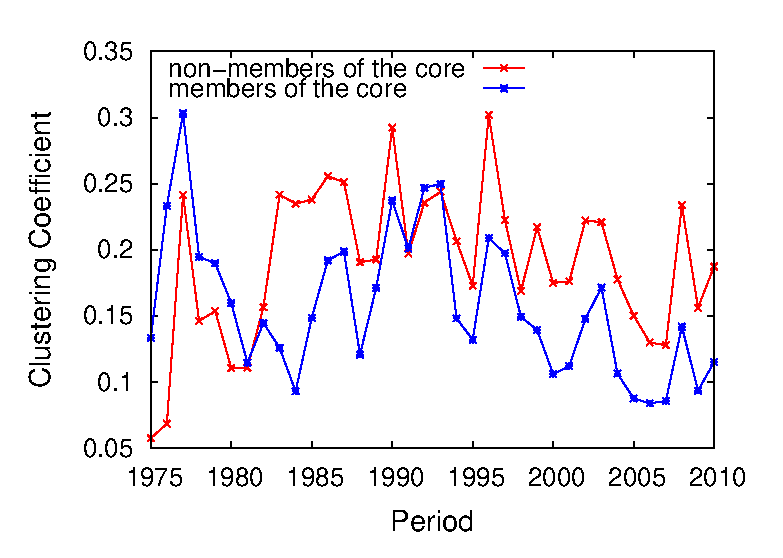
\includegraphics[scale=.33]{graficos/core_over_time/core_community/sigmod_janela_3_core_coeficiente_agrupamento.eps}
  }%
  \subfigure[\red{Avg. Degree}]{%
    \label{fig:core_com_sigmod_average_degree}
    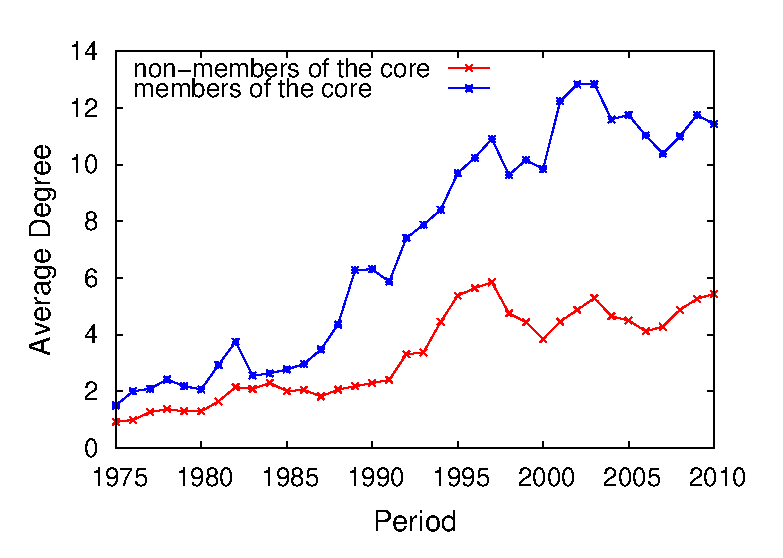
\includegraphics[scale=.33]{graficos/core_over_time/core_community/sigmod_janela_3_core_grau_medio_nodos.eps}
  }%
  \subfigure[Largest connected component]{%
    \label{fig:core_com_sigmod_largest_connected_component}
    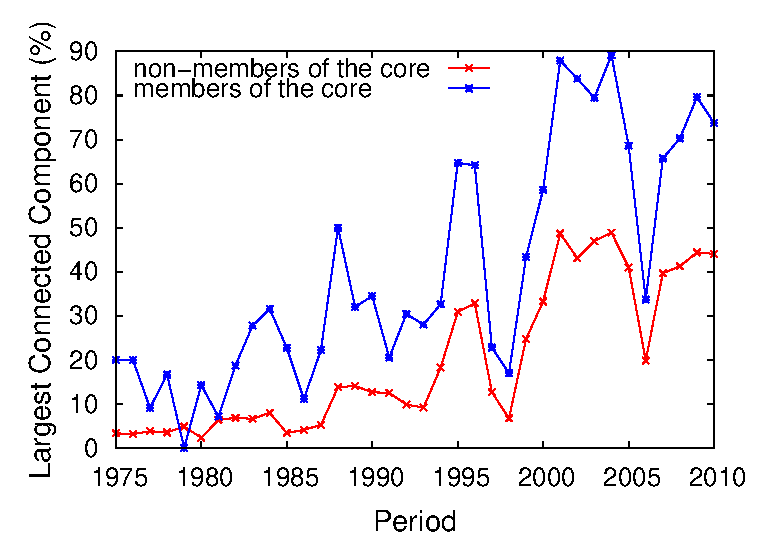
\includegraphics[scale=.33]{graficos/core_over_time/core_community/sigmod_janela_3_core_maior_componente_conectado.eps}
  }%
  \end{center}
  \caption{SIGMOD network properties for members and non-members of the core}
  \label{fig:metrics_comparing_core_community}
\end{figure*}



\subsection{Core communities and Network Structure}
\label{sub:corr}


{\bf reproduzir trabalho do rich club \cite{Xu:2010}}

We now examine to what extent the community core fluctuations affect the network structure.

\begin{figure}[!htb]
\centering
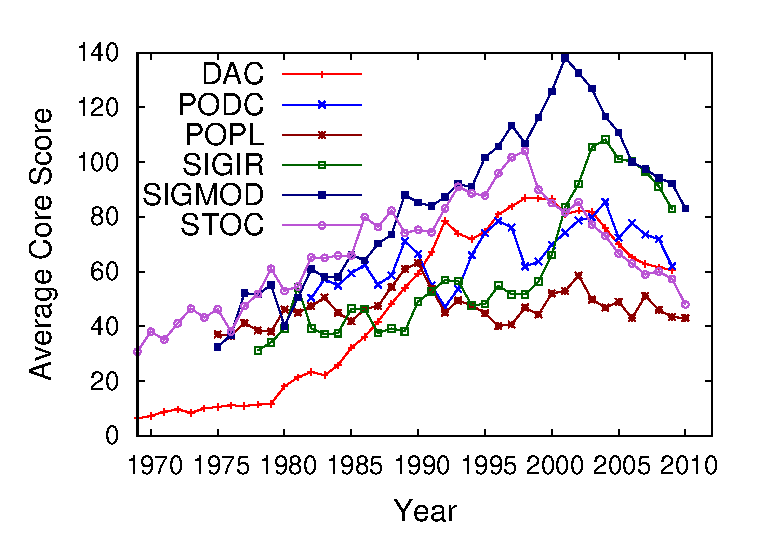
\includegraphics[scale=.5]{graficos/average_core_score/average_core_score_slide_window_grupo_temporal_web.eps}
\caption{Average Core Score}
\label{fig:average_core_score}
\end{figure}





\begin{table*}[!htb]
\centering
\caption{Corelation between average core score of the core community and the metrics of complex networks}
\label{tab:correlation_metrics}
{\small
\begin{tabular}{|l|c|c|c|c|c|c|c|} \hline
Conference & \bf Diameter & \bf Avg. Short P. & \bf Clus. Coef. & \bf Assort. & \bf Larg. WCC & \bf Avg. Deg. & \bf Num. Nodes\\ \hline
CCS & 0.34 & 0.2 & 0.23 & -0.2 & 0.45 & 0.14 & -0.13\\ \hline
CHI & 0.75 & 0.79 & -0.62 & -0.74 & 0.76 & 0.77 & 0.58\\ \hline
CIKM & 0.56 & 0.56 & -0.52 & -0.67 & 0.39 & 0.87 & 0.64\\ \hline
DAC & 0.8 & 0.85 & -0.49 & -0.63 & 0.76 & 0.92 & 0.84\\ \hline
HSCC & 0.17 & 0.45 & -0.62 & -0.71 & 0.87 & 0.55 & -0.55\\ \hline
ICSE & 0.81 & 0.83 & -0.52 & -0.84 & 0.68 & 0.8 & 0.78\\ \hline
ISCA & 0.63 & 0.55 & 0.54 & -0.32 & 0.63 & 0.81 & 0.41\\ \hline
ISSAC & 0.05 & 0.01 & -0.25 & -0.43 & -0.07 & 0.21 & 0.78\\ \hline
KDD & 0.1 & 0.17 & -0.33 & -0.67 & 0.2 & 0.14 & 0.2\\ \hline
MICRO & 0.35 & 0.35 & 0.28 & -0.36 & 0.52 & 0.51 & 0.36\\ \hline
MOBICOM & -0.04 & 0.11 & 0.13 & -0.65 & 0.23 & -0.09 & 0.02\\ \hline
Multimedia & 0.67 & 0.68 & -0.91 & -0.95 & 0.67 & 0.69 & 0.75\\ \hline
PODC & 0.4 & 0.42 & -0.23 & -0.2 & 0.13 & 0.68 & 0.57\\ \hline
POPL & 0.21 & 0.2 & 0.23 & -0.43 & 0.25 & 0.19 & 0.05\\ \hline
SAC & 0.48 & 0.59 & 0.16 & -0.39 & -0.55 & 0.16 & 0.23\\ \hline
SIGCOMM & 0.18 & 0.19 & 0.05 & -0.81 & 0.49 & 0.41 & -0.03\\ \hline
SIGCSE & 0.88 & 0.84 & -0.22 & -0.5 & 0.93 & 0.87 & 0.8\\ \hline
SIGDOC & 0.73 & 0.78 & -0.36 & -0.89 & 0.66 & 0.76 & 0.05\\ \hline
SIGGRAPH & 0.79 & 0.85 & -0.45 & -0.75 & 0.94 & 0.88 & 0.55\\ \hline
SIGIR & 0.83 & 0.85 & -0.42 & -0.77 & 0.7 & 0.89 & 0.88\\ \hline
SIGMETRICS & 0.31 & 0.24 & 0.3 & -0.44 & 0.37 & 0.64 & 0.43\\ \hline
SIGMOD & 0.78 & 0.81 & 0.27 & -0.61 & 0.77 & 0.87 & 0.68\\ \hline
SIGUCCS & 0.38 & -0.22 & 0.53 & -0.13 & 0.51 & 0.7 & 0.57\\ \hline
STOC & 0.61 & 0.63 & 0.54 & -0.37 & 0.82 & 0.88 & 0.68\\ \hline
{\bf Average} & {\bf 0.49} & {\bf 0.49} & {\bf -0.11} & {\bf -0.56} & {\bf 0.5} & {\bf 0.59} & {\bf 0.42}\\ \hline
\end{tabular}
}
\end{table*}



